\documentclass[UTF8]{article}
\usepackage{ctex}
\usepackage{geometry}
\geometry{a4paper,scale=0.8}
\usepackage{listings}
\usepackage{fontspec}
\newfontfamily\jetbrains{JetBrains Mono}
\lstset{
    breaklines,                                 % 自动将长的代码行换行排版
    extendedchars=false,                        % 解决代码跨页时,章节标题,页眉等汉字不显示的问题
    backgroundcolor=\color[rgb]{0.96,0.96,0.96},% 背景颜色
    keywordstyle=\color{blue}\bfseries,         % 关键字颜色
    identifierstyle=\color{black},              % 普通标识符颜色
    commentstyle=\color[rgb]{0,0.6,0},          % 注释颜色
    stringstyle=\color[rgb]{0.58,0,0.82},       % 字符串颜色
    showstringspaces=false,                     % 不显示字符串内的空格
    numbers=left,                               % 显示行号
    numberstyle=\tiny\jetbrains,                    % 设置数字字体
    basicstyle=\small\jetbrains,                    % 设置基本字体
    captionpos=t,                               % title在上方(在bottom即为b)
    frame=single,                               % 设置代码框形式
    rulecolor=\color[rgb]{0.8,0.8,0.8},         % 设置代码框颜色
}
\usepackage{hyperref}
\hypersetup{
    hypertex=true,
    colorlinks=true,
    linkcolor=black,
    anchorcolor=black,
    citecolor=black,
}
\usepackage{graphicx}
\usepackage{float}
\usepackage{bookmark}

\title{Verilog实验 lab2实验报告}
\author{PB19071405 王昊元}
\date{2022 年 04 月 11 日}

\begin{document}
    \maketitle
    \section{实验目的}
    \begin{enumerate}
        \item 掌握五级流水线CPU的设计方法
        \item 熟悉RISC-V的指令集和数据通路,了解其设计背后的思想
        \item 进一步提高使用verilog编码和调试的能力,学会使用仿真(Simulation)调试
    \end{enumerate}
    \section{实验要求}
    \begin{enumerate}
        \item 实现可以处理基本指令的五级流水线,需实现指令包括:SLLI、SRLI、SRAI、ADD、SUB、SLL、SLT、SLTU、XOR、SRL、SRA、OR、AND、ADDI、SLTI、SLTIU、XORI、ORI、ANDI、LUI、AUIPC
        \item 实现可以处理数据相关的五级流水线,需实现指令包括:JALR、LB、LH、LW、LBU、LHU、SB、SH、SW、BEQ、BNE、BLT、BLTU、BGE、BGEU、JAL
        \item 实现CSR数据通路及相关指令,指令包括:CSRRW、CSRRS、CSRRC、CSRRWI、CSRRSI、CSRRCI
    \end{enumerate}
    \section{实验核心实现}
    \begin{enumerate}
        \item 第一阶段:实现基本指令,不考虑数据相关 \\
        这一部分主要是补全各个模块,使得流水线能够实现基本指令,各个模块的功能也都很独立,按照其对应功能实现即可。 \\
        需要提及的有ALU中的{\jetbrains NAND}计算,我在完成第一阶段时,没有认真做研究,将该运算实现为与非,
        但在完成第三阶段CSR的相关实现时,我才发现{\jetbrains NAND}的目的在于清除某些位
        (对应{\jetbrains CSRRC}和{\jetbrains CSRRCI}指令),也就是需要实现为
        {\jetbrains ALU\_out = \textasciitilde op1 \& op2;}。\\
        控制模块也很重要,不过由于在第一阶段不需要考虑数据相关和CSR相关指令,
        所以这一部分的控制模块只是根据指令的性质(如是否写寄存器、ALU的数据来源、立即数的类型等)
        完成这一部分指令的控制。
        \item 第二阶段:实现跳转指令,考虑数据相关 \\
        这一部分主要需要完成三个部分,{\jetbrains BranchDecision}、{\jetbrains DataExtend}和相关的控制信号。 \\
        Br指令只需要在模块中根据不同的指令进行判断是否跳转,输出信号即可;数据扩展模块只需要根据不同的指令对数据进行不同的扩展即可。
        控制模块中,{\jetbrains load\_type}要根据不同的LOAD指令输出不同的控制信号,
        {\jetbrains br\_type}要根据不同的Branch指令输出不同的信号,
        {\jetbrains jal}和{\jetbrains jalr}信号则根据指令是否为JAL和JALR判断。\\
        此外需要注意的点有JAL指令为J类立即数,而JALR指令为I类立即数;
        JAL指令和JALR指令都需要将{\jetbrains PC+4}写回寄存器,故{\jetbrains reg\_write\_en}信号为1。
        \item 第三阶段:实现CSR数据通路及相关指令 \\
        完成这一部分首先需要对CSR的六条指令有所了解,才能正确实现指令、数据通路及控制信号。 \\
        \begin{table}[H]
            \centering
            \caption{CSR相关指令}
            \scalebox{0.8}
            {
                \begin{tabular}{|c||c|c||c|}
                    \hline
                    指令 & 操作内容 & ALU操作类型 & 数据来源 \\
                    \hline
                    CSRRW & Atomic Read/Write CSR & OP1(将OP1往下一阶段传递,最后写CSR) & 寄存器数据 \\
                    \hline
                    CSRRWI & Atomic Read/Write CSR & OP1(将OP1往下一阶段传递,最后写CSR) & 立即数 \\
                    \hline
                    CSRRS & Atomic Read and Set Bits in CSR & OR(实现置位操作) & 寄存器数据 \\
                    \hline
                    CSRRSI & Atomic Read and Set Bits in CSR & OR(实现置位操作) & 立即数 \\
                    \hline
                    CSRRC & Atomic Read and Clear Bits in CSR & NAND(实现清除操作) & 寄存器数据 \\
                    \hline
                    CSRRCI & Atomic Read and Clear Bits in CSR & NAND(实现清除操作) & 立即数 \\
                    \hline
                \end{tabular}
            }
            \label{csr table}
        \end{table}
        从表\ref{csr table}可知各个指令的控制信号。 \\
        另外值得一提的是,因为CSR指令是根据指令的前12位(即{\jetbrains inst[31:20]})来寻址,
        故CSR寄存器设置4096个即可。
    \end{enumerate}
    \section{实验结果及分析}
    各个测试程序的仿真结果如下:\\
    \begin{figure}[H]
        \centering
        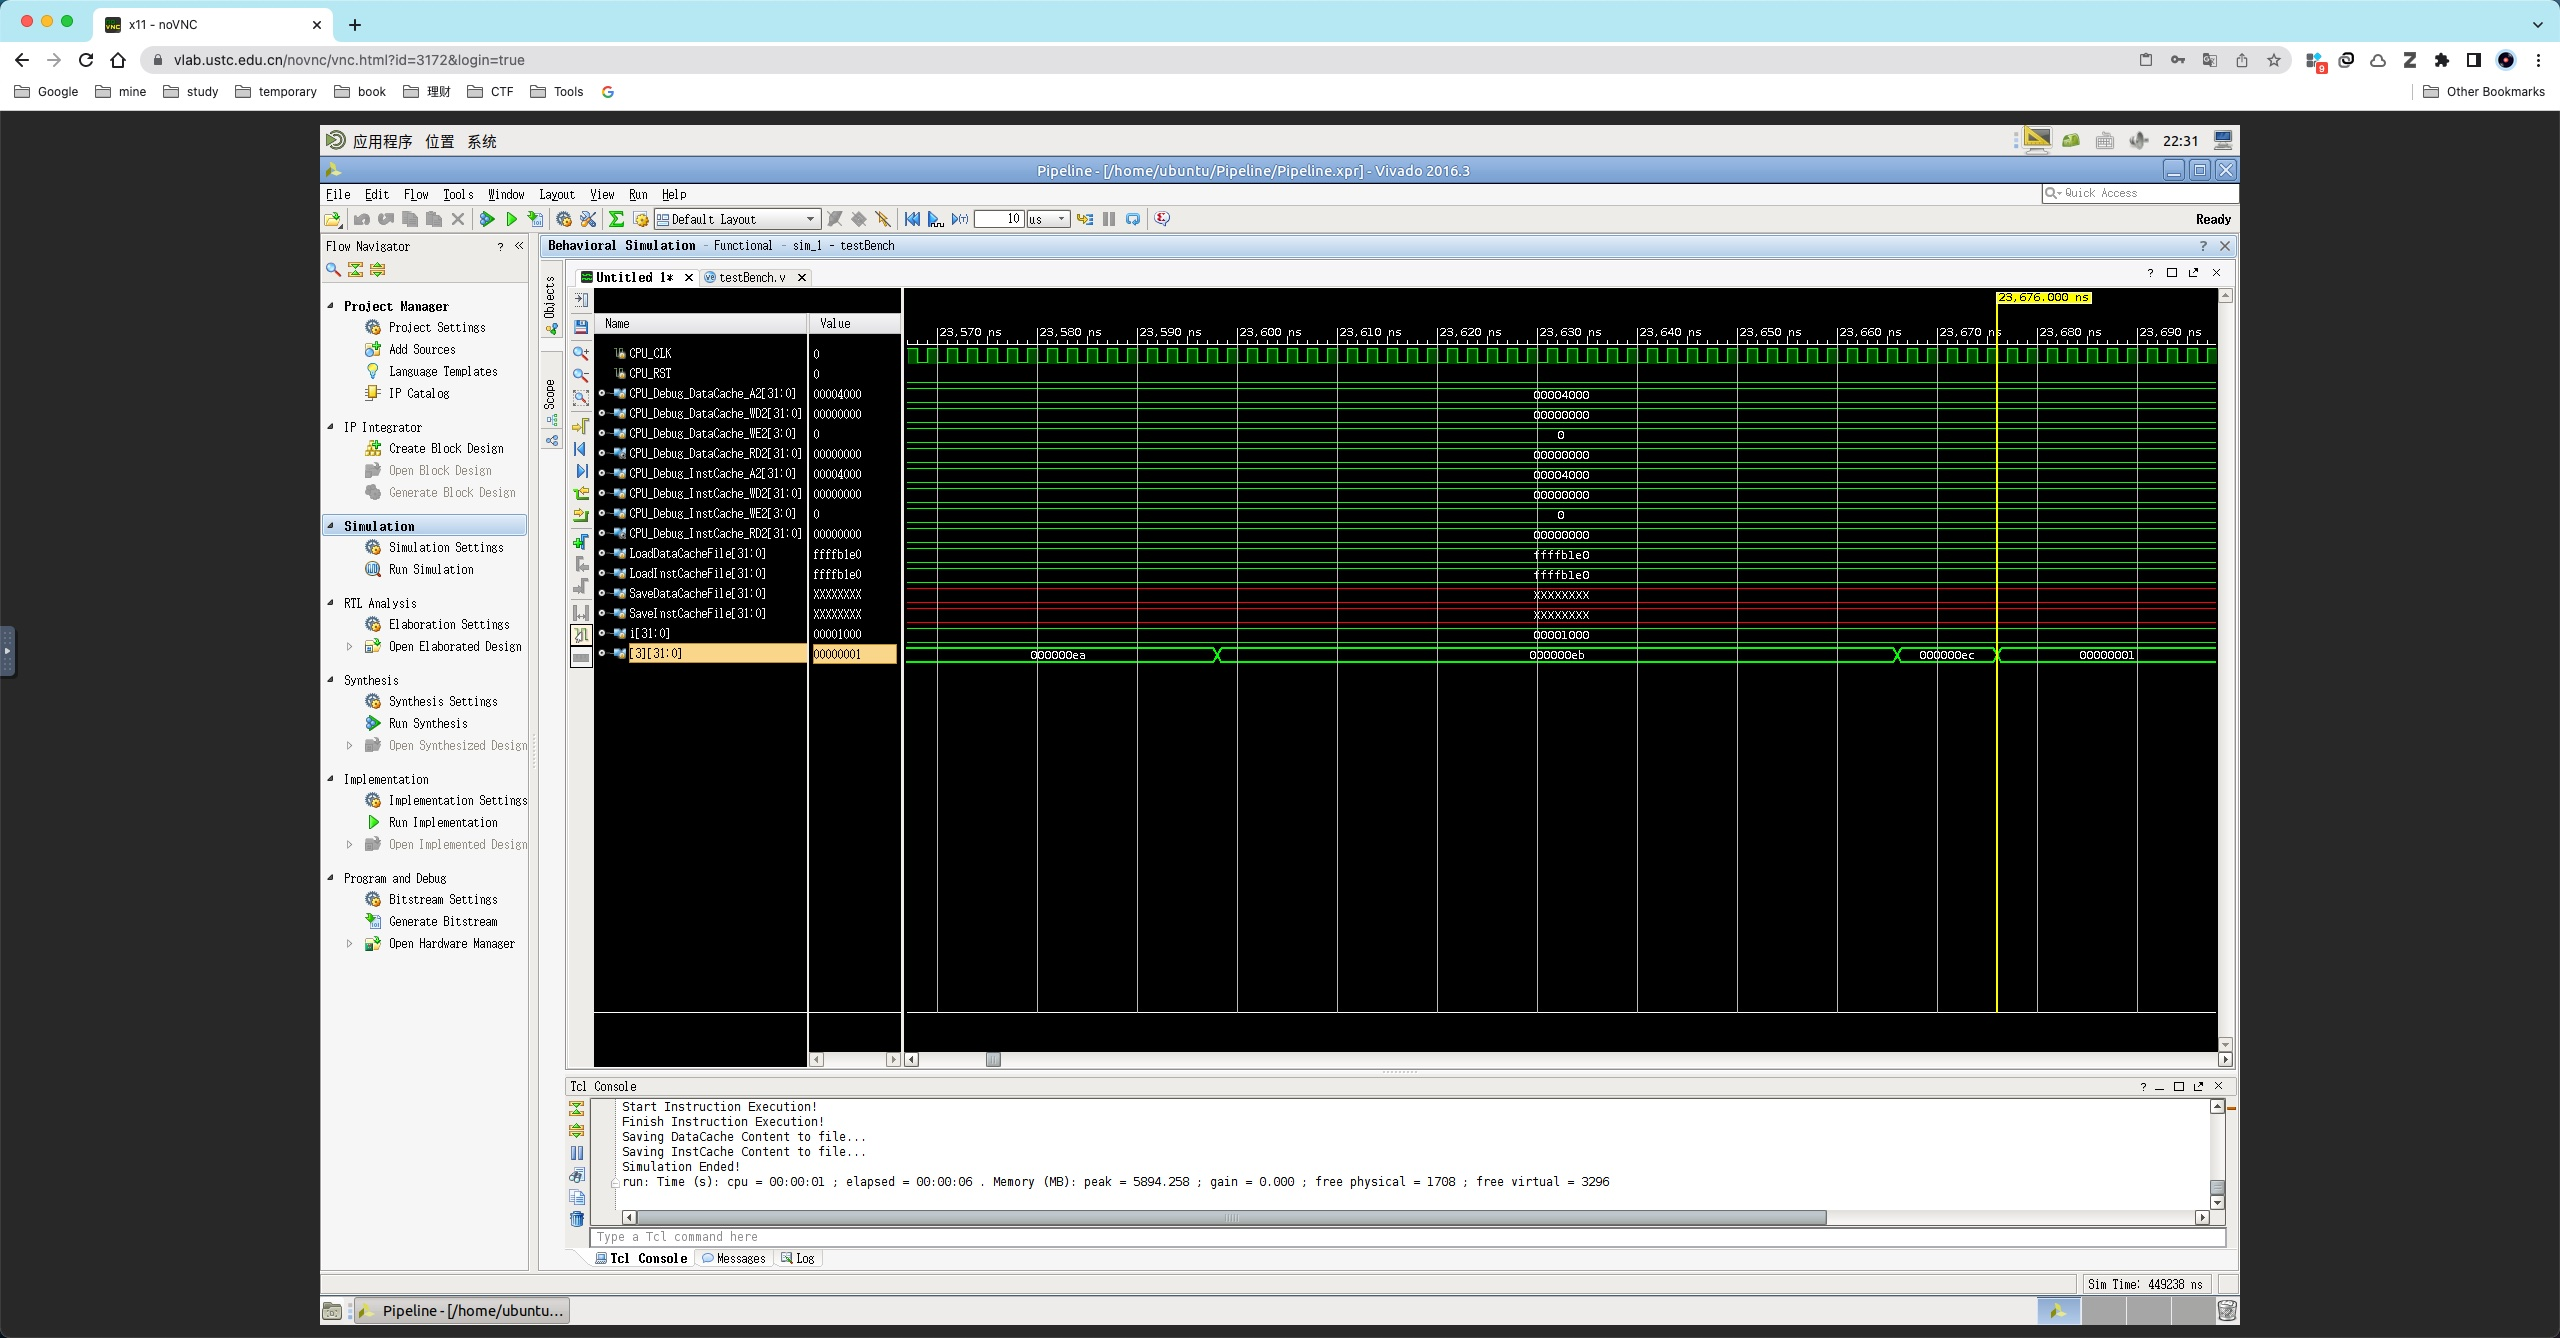
\includegraphics[width=0.7\textwidth]{./figs/test1_result.jpg}
        \caption{测试1结果}
        \label{test1}
    \end{figure}
    \begin{figure}[H]
        \centering
        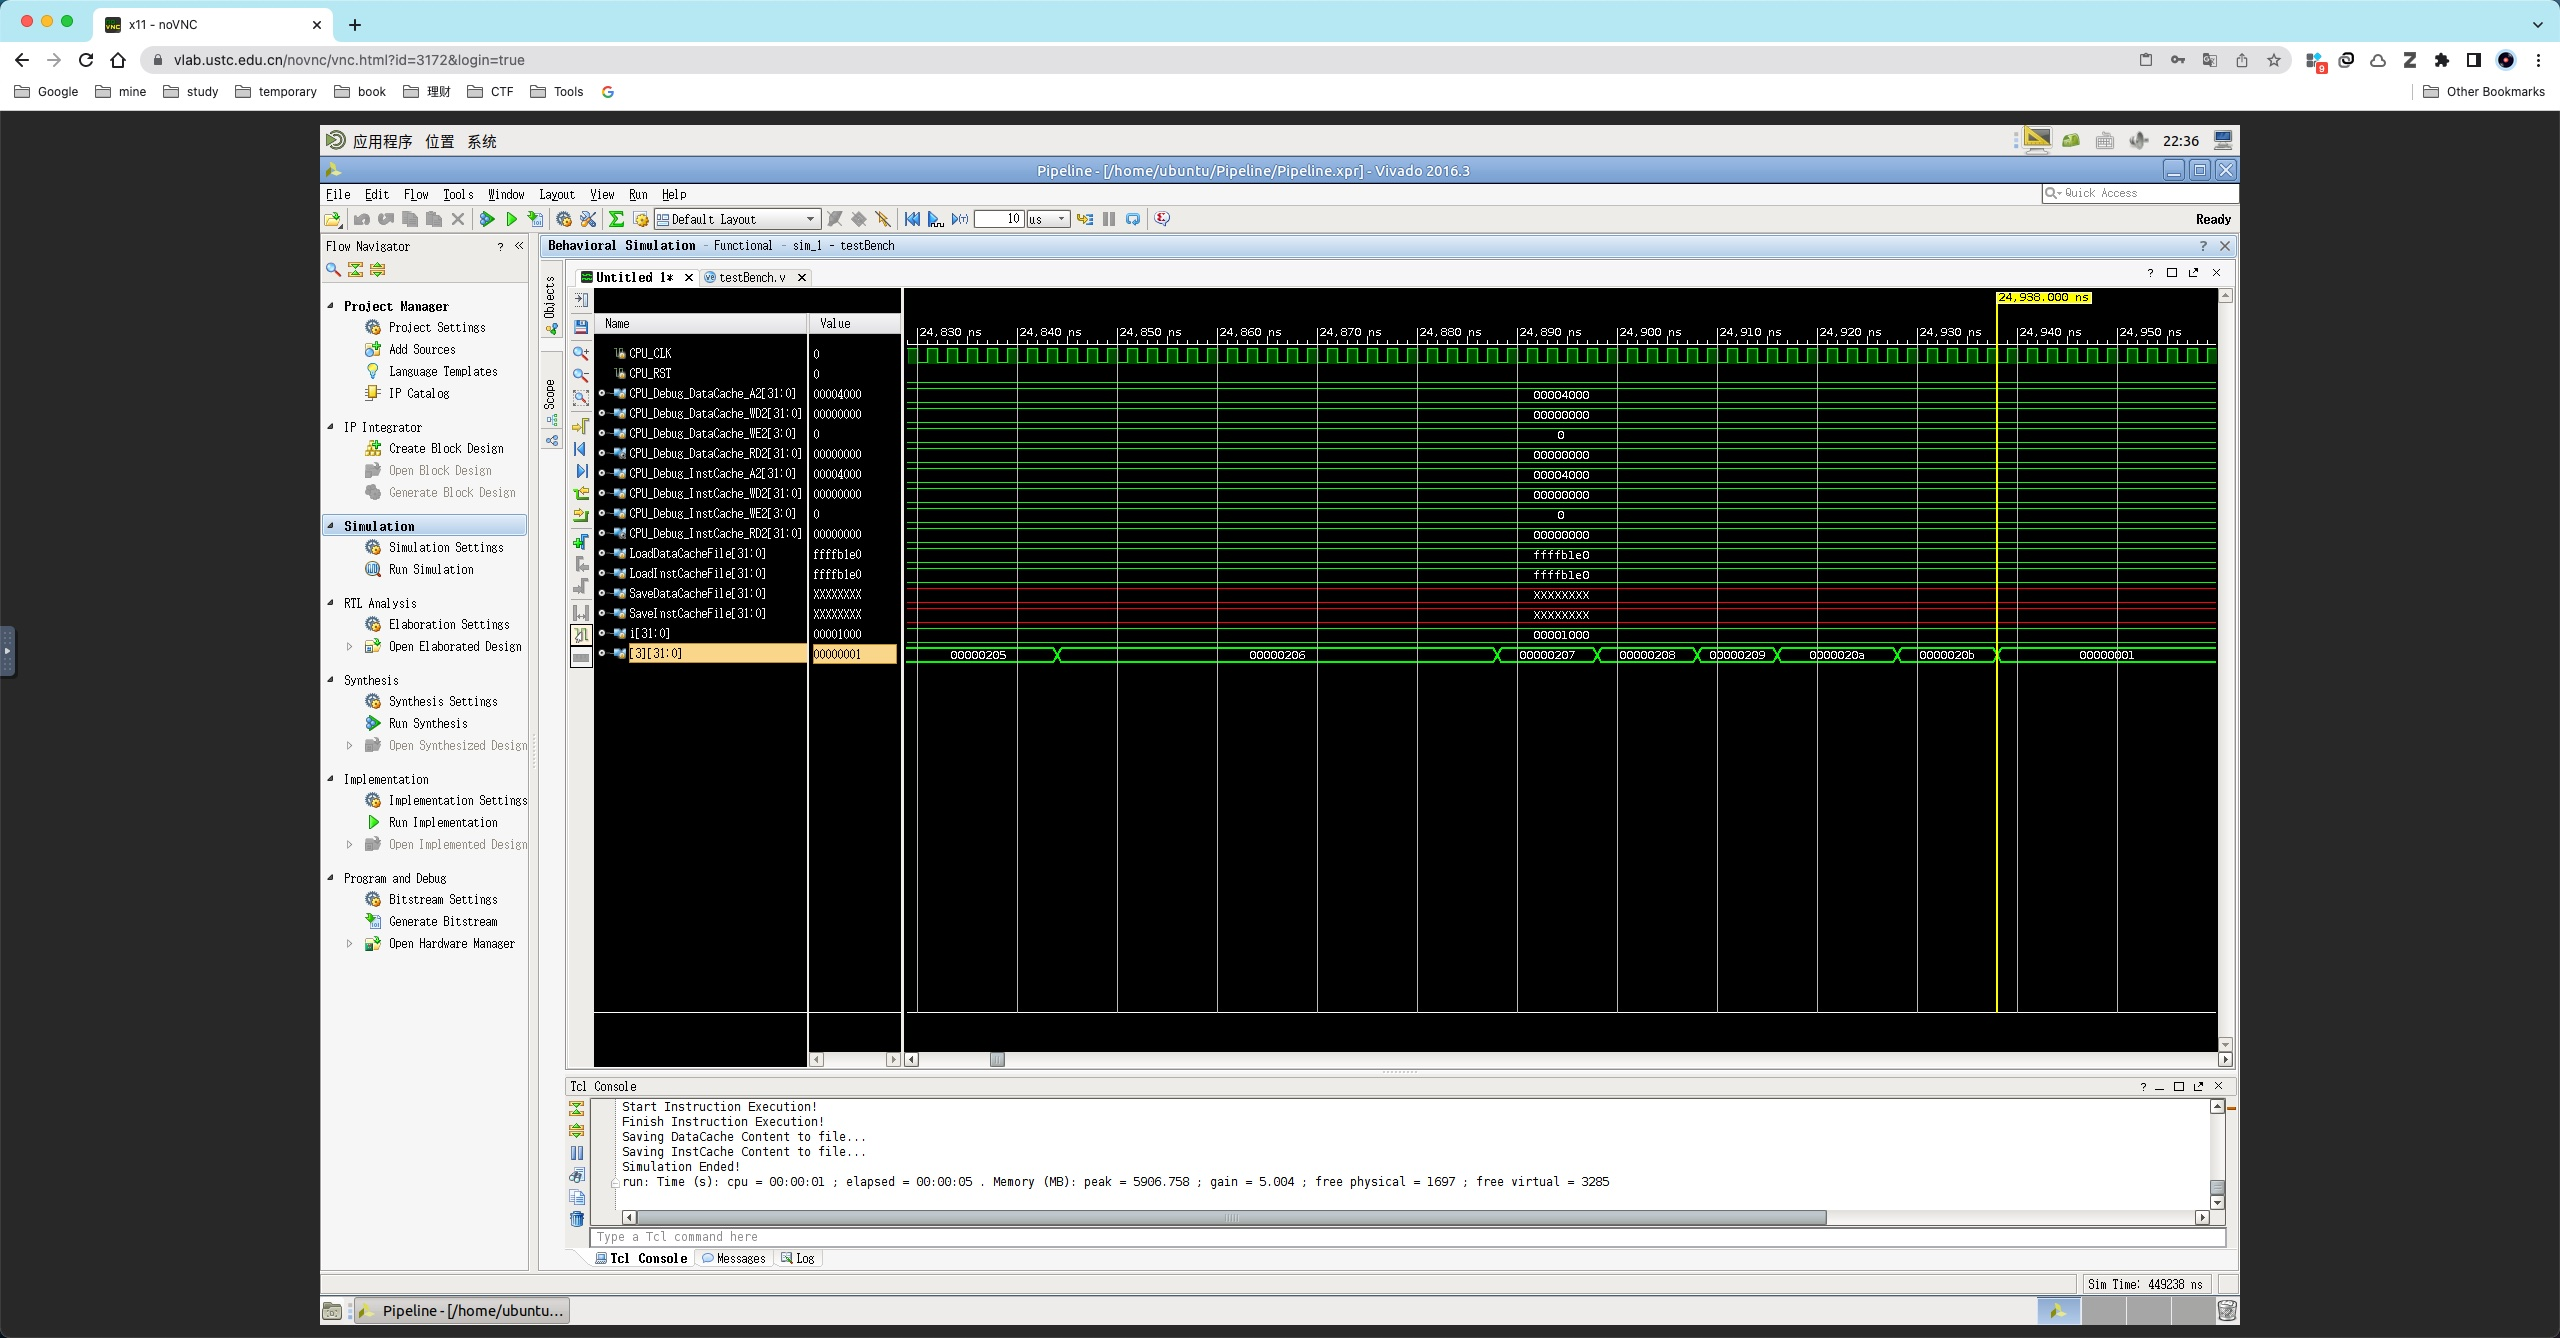
\includegraphics[width=0.7\textwidth]{./figs/test2_result.jpg}
        \caption{测试2结果}
        \label{test2}
    \end{figure}
    \begin{figure}[H]
        \centering
        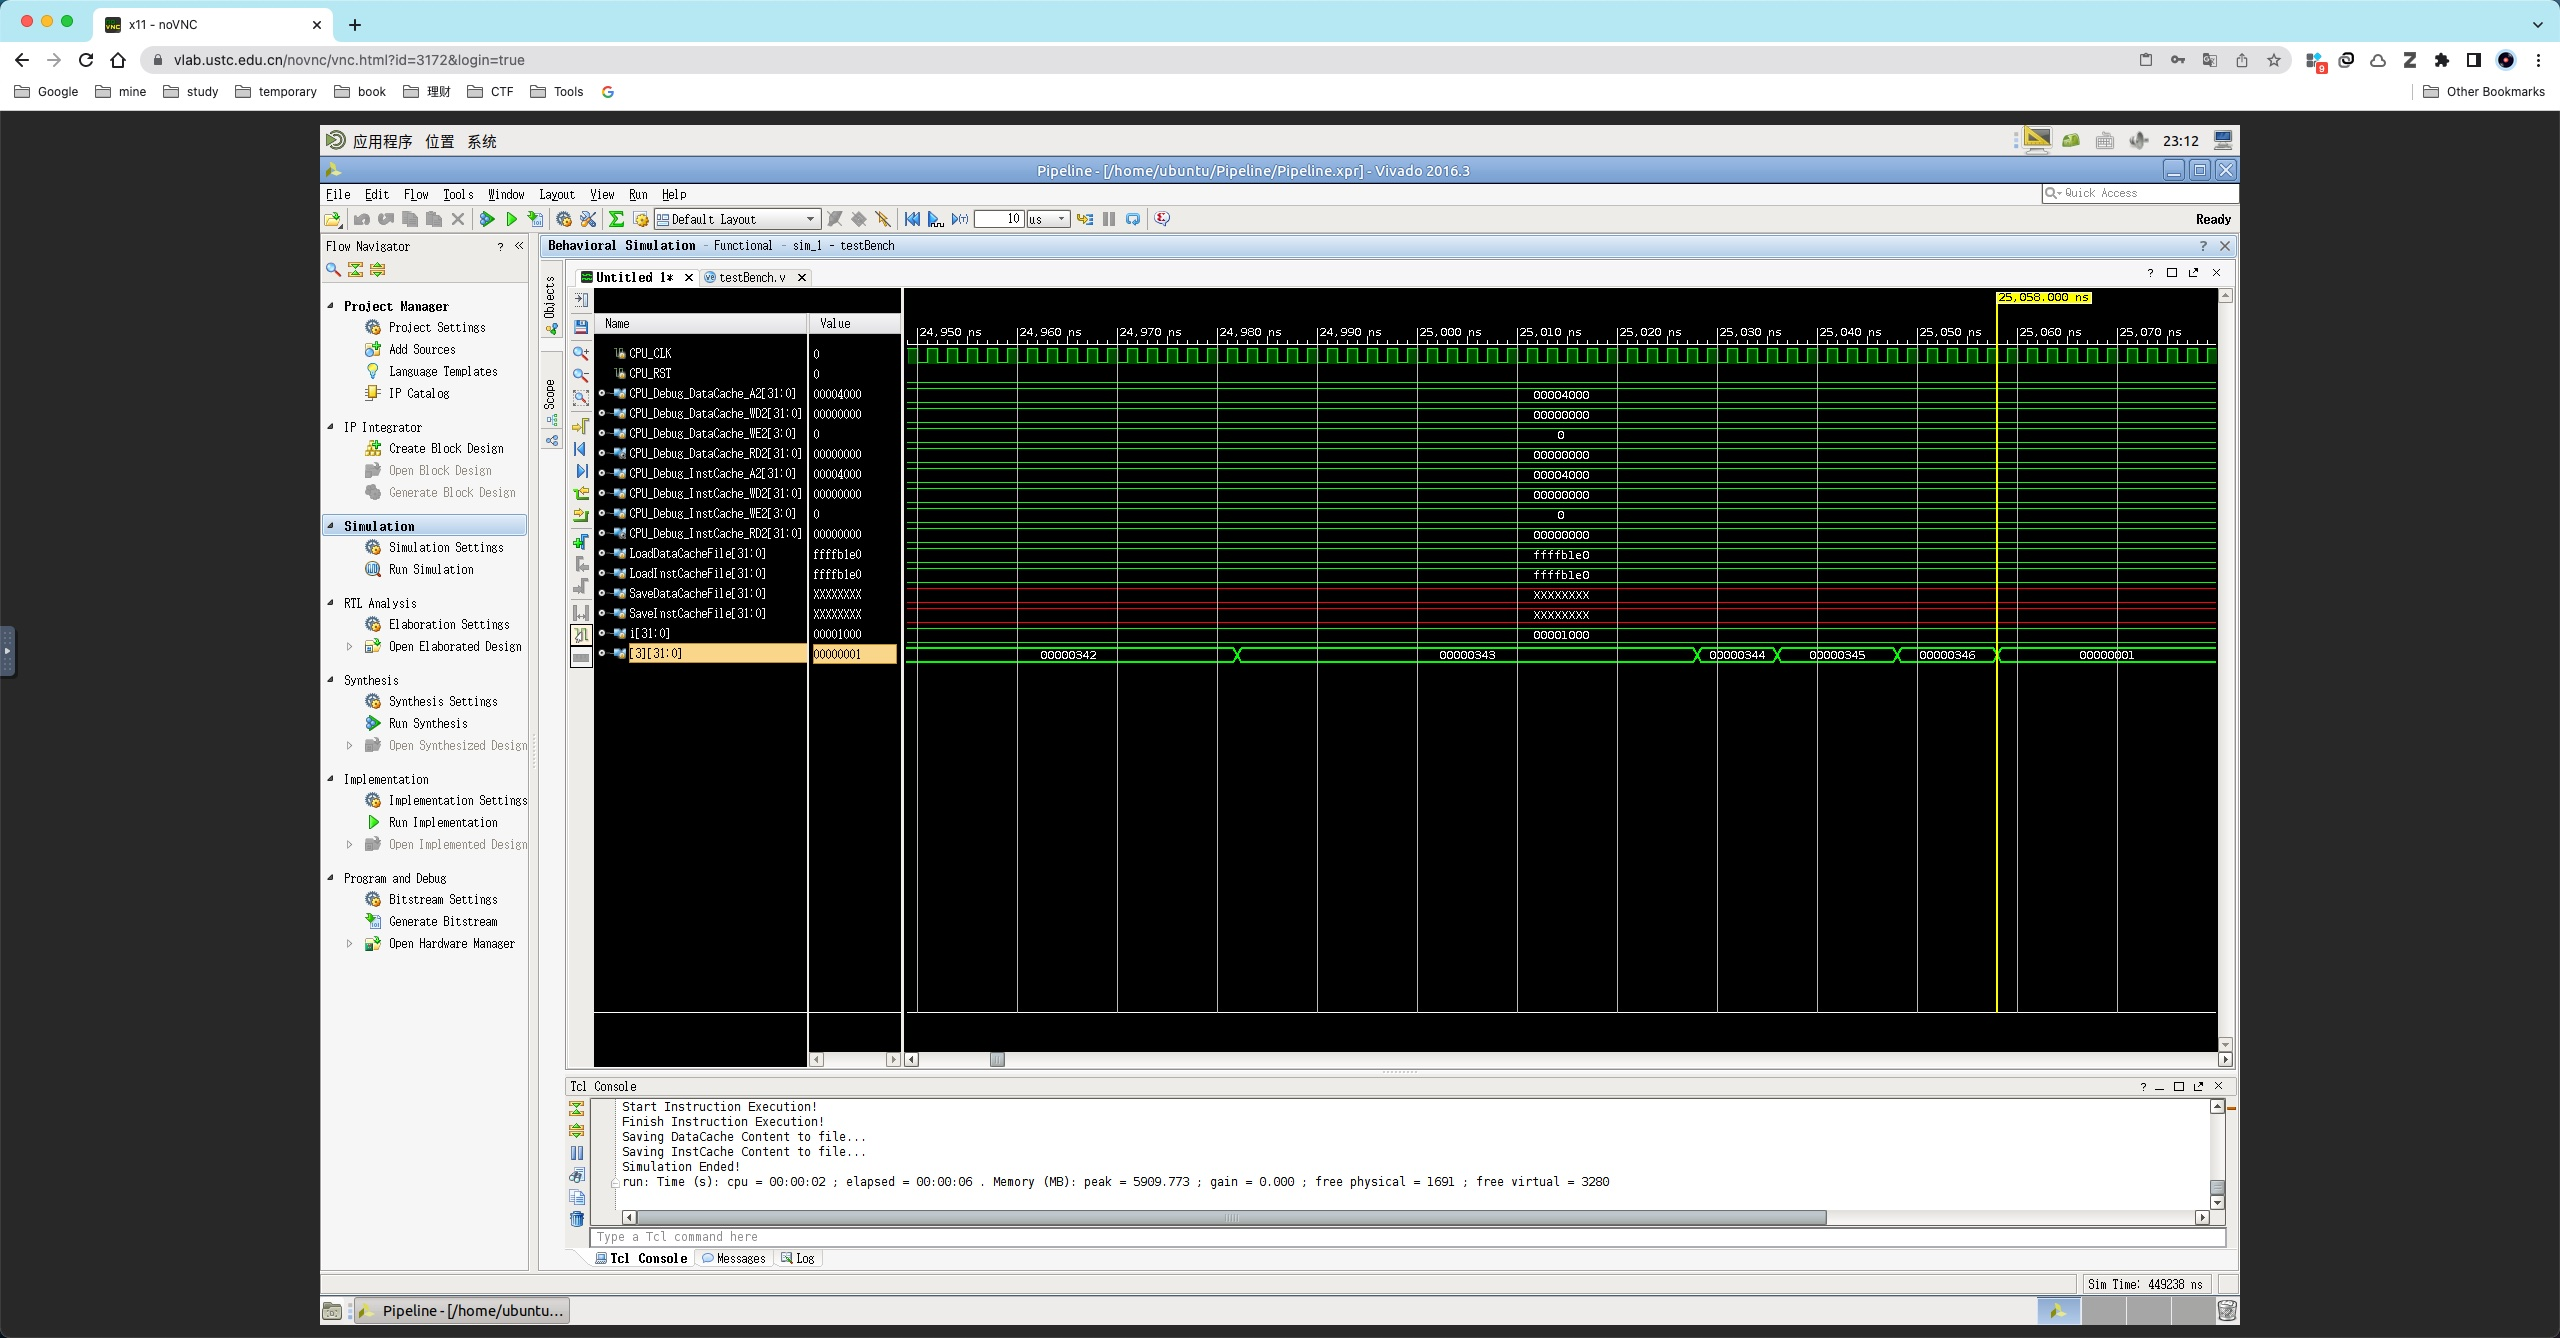
\includegraphics[width=0.7\textwidth]{./figs/test3_result.jpg}
        \caption{测试3结果}
        \label{test3}
    \end{figure}
    \begin{figure}[H]
        \centering
        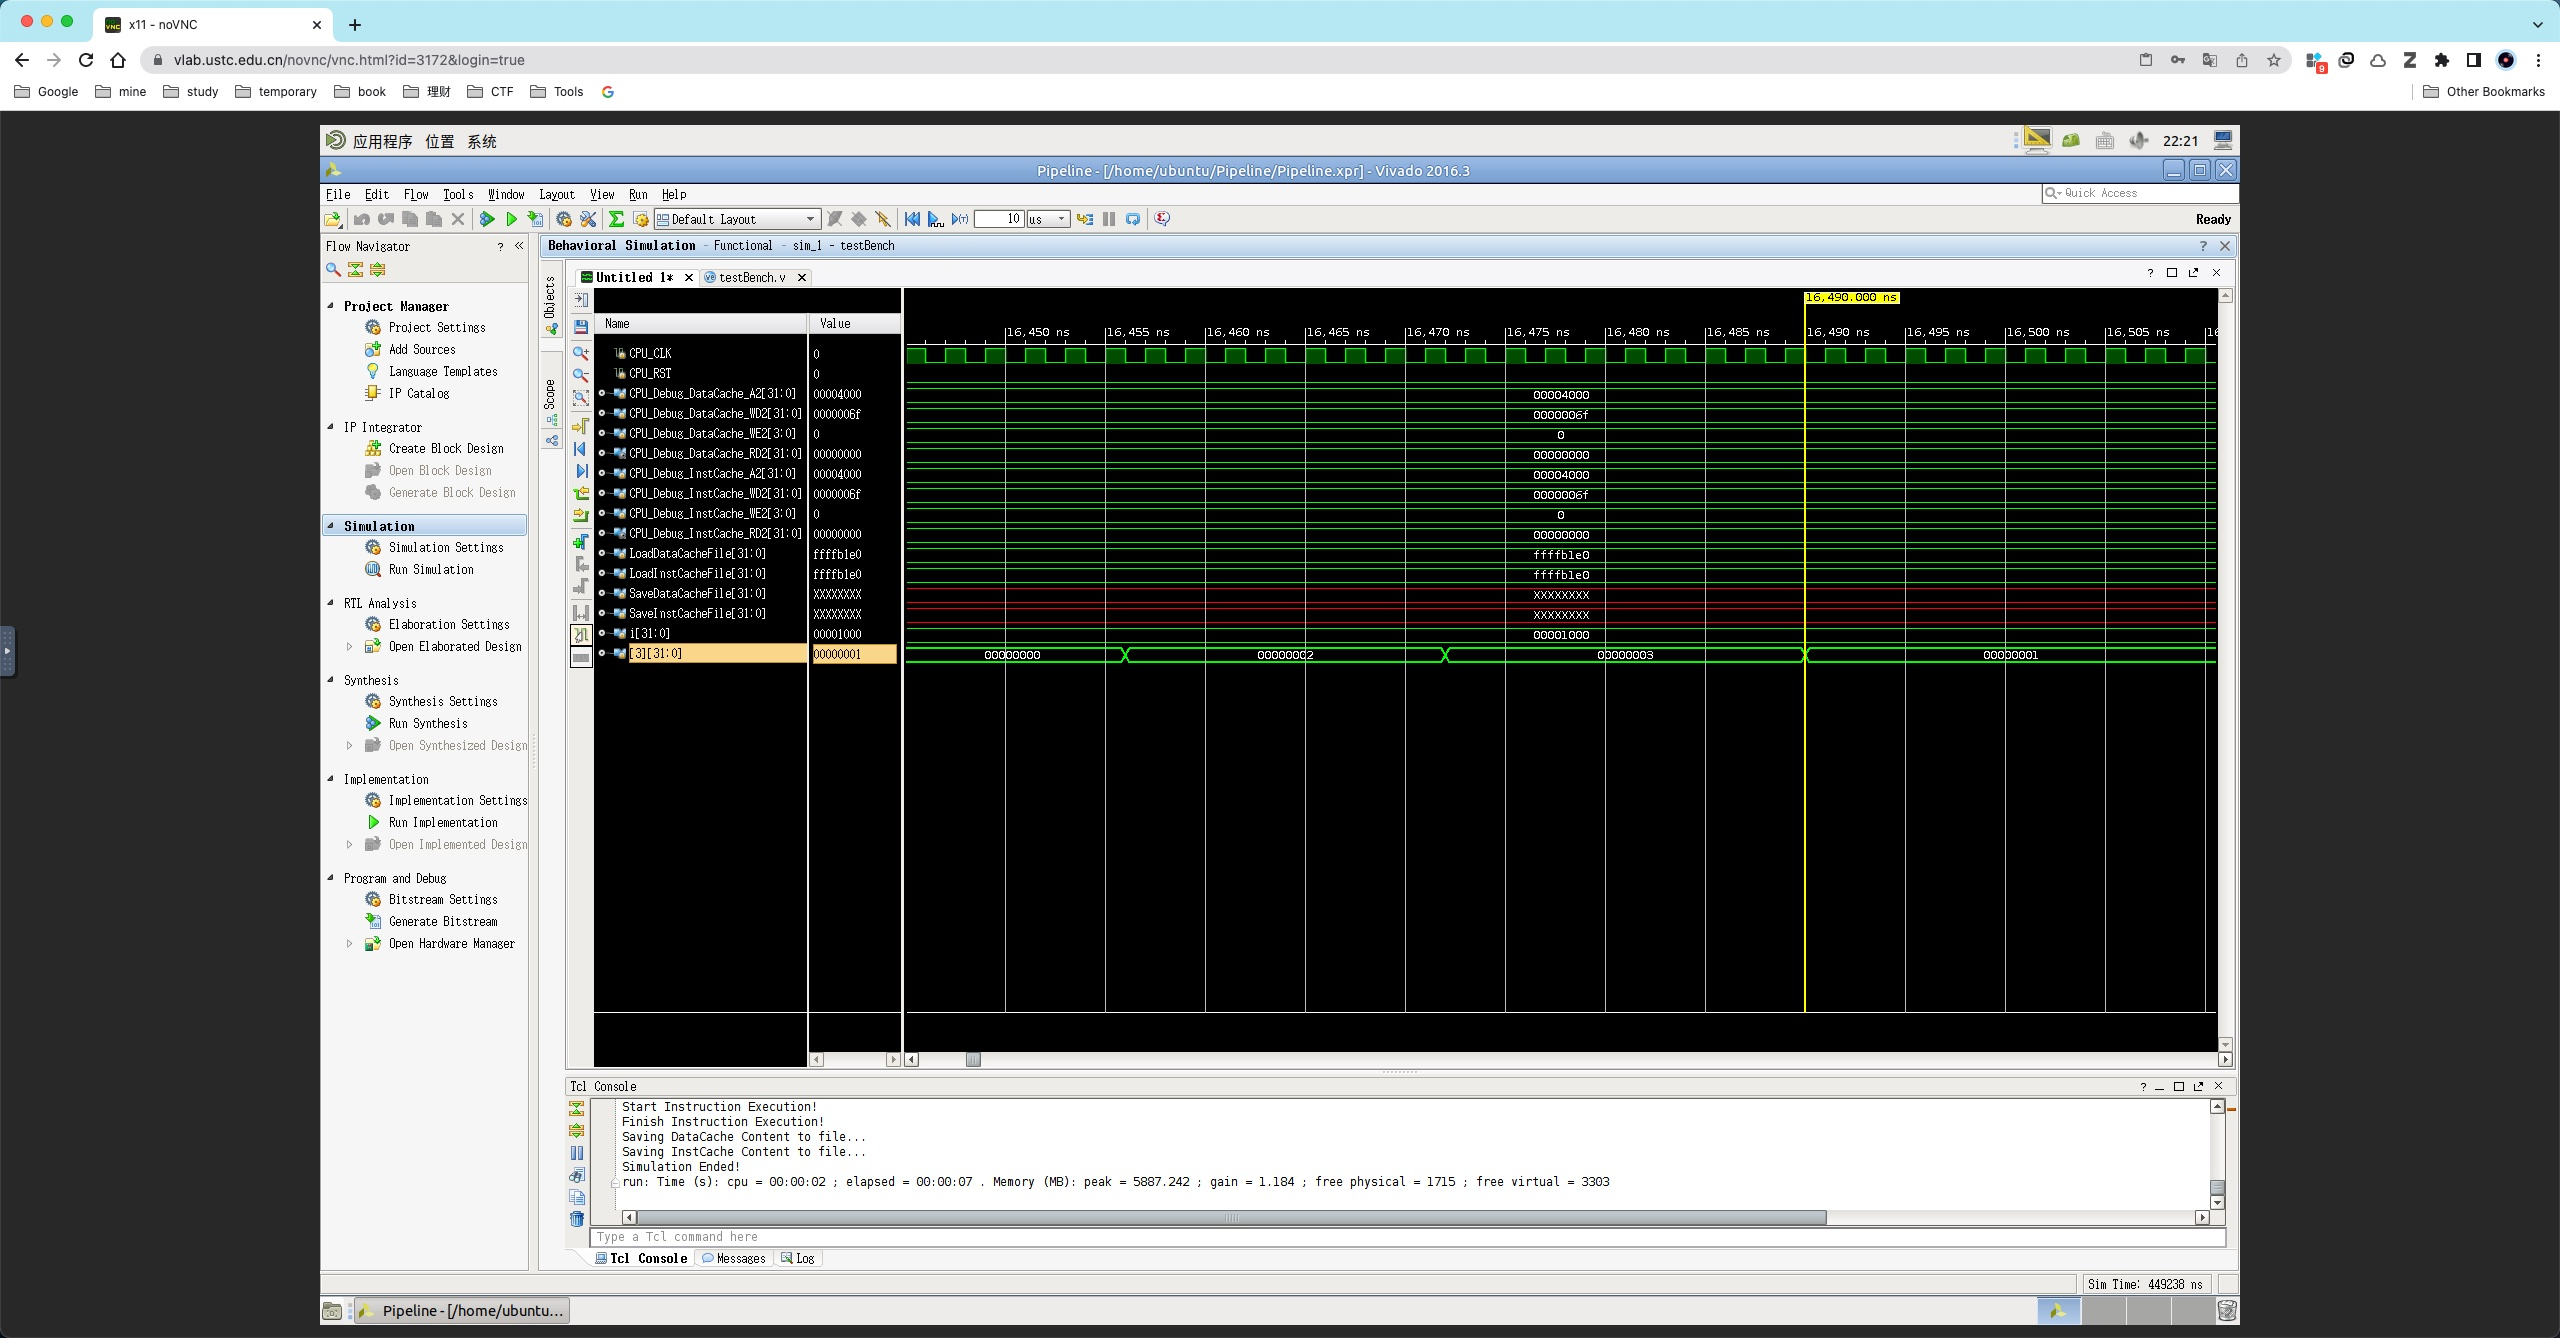
\includegraphics[width=0.7\textwidth]{./figs/csr_result.jpg}
        \caption{CSR测试结果}
        \label{csr test}
    \end{figure}
    从以上各图可以看到,3号寄存器最后都变为1,这意味着流水线通过了各项测试,完成了实验的各项要求。
    \section{实验总结}
    \begin{enumerate}
        \item 通过本次实验,我对RISCV各种指令的熟悉程度与理解更加深刻,
        同时也对流水线的细节也更加了解,比如流水线的基本模式、旁路转发、数据冲突导致的流水线停顿等等。
        \item 此外,我更加熟悉了Vivado的仿真功能,对其也有了更深入的了解,
        也开始尝试使用终端输出来使得Debug更加方便。
        \item 在完成实验的过程中,我还回顾熟悉了Verilog语言的使用与编写,
        同时也可以利用Vivado的仿真结果进行错误分析,逐步确定Bug的位置,从而修复问题,完成实验。
    \end{enumerate}

\end{document}